%
%                       This is a basic LaTeX Template
%                       for the Informatics Research Review

\documentclass[a4paper,11pt]{article}
% Add local fullpage and head macros
\usepackage{head,fullpage}     
% Add graphicx package with pdf flag (must use pdflatex)
\usepackage[pdftex]{graphicx}  
% Better support for URLs
\usepackage{url}
% Date formating
\usepackage{datetime}
% For Gantt chart
\usepackage{pgfgantt}
\usepackage{xcolor}
\usepackage[utf8]{inputenc}

\newdateformat{monthyeardate}{%
  \monthname[\THEMONTH] \THEYEAR}

\parindent=0pt          %  Switch off indent of paragraphs 
\parskip=5pt            %  Put 5pt between each paragraph  
\Urlmuskip=0mu plus 1mu %  Better line breaks for URLs


%                       This section generates a title page
%                       Edit only the following three lines
%                       providing your exam number, 
%                       the general field of study you are considering
%                       for your review, and name of IRR tutor

\newcommand{\examnumber}{B138630}
\newcommand{\field}{Finding the Right Teacher for a Difficult Student}
\newcommand{\tutor}{Stuart Anderson}
\newcommand{\supervisor}{Amos Storkey co-supervised by Elliot Crowley}

\begin{document}
\begin{minipage}[b]{110mm}
        {\Huge\bf School of Informatics
        \vspace*{17mm}}
\end{minipage}
\hfill
\begin{minipage}[t]{40mm}               
        \makebox[40mm]{
        \includegraphics[width=40mm]{crest.png}}
\end{minipage}
\par\noindent
    % Centre Title, and name
\vspace*{2cm}
\begin{center}
        \Large\bf Informatics Project Proposal \\
        \Large\bf \field
\end{center}
\vspace*{1.5cm}
\begin{center}
        \bf \examnumber\\
        \monthyeardate\today
\end{center}
\vspace*{5mm}

%
%                       Insert your abstract HERE
%                       
\begin{abstract}
        Network distillation can improve the performance of a neural network through distilling the knowledge of a teacher network into a student. The teacher network is usually large and deep, whilst the student is much smaller. Typically, network distillation is effective where the teacher and student architectures are standard, off-the-shelf architectures. This proposal suggests an investigation into network distillation techniques in cases where the student network is of some non-standard architecture developed through Neural Architecture Search. We suggest experimental work investigating the performance of standard teachers for non-standard students, as well as work on modelling a teacher from a given student.
\end{abstract}

\vspace*{1cm}

\vspace*{3cm}
Date: \today

\vfill
{\bf Tutor:} \tutor\\
{\bf Supervisor:} \supervisor
\newpage

%                                               Through page and setup 
%                                               fancy headings
\setcounter{page}{1}                            % Set page number to 1
\footruleheight{1pt}
\headruleheight{1pt}
\lfoot{\small School of Informatics}
\lhead{Informatics Research Review}
\rhead{- \thepage}
\cfoot{}
\rfoot{Date: \date{\today}}
%
\tableofcontents                                % Makes Table of Contents
\section{Motivation}
\label{sec:motivation}
In Network Distillation \cite{ba2014deep} \cite{hinton2015distilling} learnt representations from a \textit{teacher} network are used to improve the performance of a \textit{student} network. The teacher network is typically a large, deep network that performs very well on a given task. The student network is usually much shallower (with some exceptions \cite{furlanello2018born}), and when trained on just the original labelled data does not perform as well as the teacher. The student network utilises the learnt representations of the teacher network to improve its performance. To do this, there are two standard approaches: \textit{Knowledge Distillation}, and \textit{Attention Transfer}. Knowledge Distillation attempts to produce outputs that are similar to the teacher network, whilst still minimising its own loss between its output and the target labels. Attention transfer encourages the distribution of the teacher and student activations at specified layers to be similar,  whilst also minimising the loss between its output and the target labels. 

As well as improving performance of a student network by the introduction of a teacher network, network distillation can also be considered in a network-compression perspective. In network-compression we attempt to obtain similar performance in the student network as in the teacher, however, the student network is much smaller than the original teacher. Effectively compressing a network is a very useful task. The performance of deep neural networks is largely limited by the number of learnable parameters in the network \cite{lecun2015deep}, motivating the development of very deep networks \cite{shazeer2017outrageously}. However, whilst deep networks can be very effective, they require large amounts of memory to be stored, as well as huge amounts of compute power to train. Network distillation addresses this problem by maintaining the performance of the larger network whilst having a smaller memory footprint. 

An important question within network distillation is how to best determine the architectures for these teacher and student networks. In cases where the student is a standard, off-the-shelf architecture (e.g. ResNet \cite{he2016deep}, DenseNet \cite{huang2017densely}), a teacher of that same architecture can be used \cite{crowley2018moonshine}. However, in cases where the student is very non-standard, it becomes difficult to determine an effective architecture for the teacher. If the student network is the product of some \textit{Neural Architecture Search} (NAS) algorithm (e.g. \cite{liu2018darts} \cite{zoph2018learning}), then determining a good teacher architecture becomes even more challenging. This project aims to tackle the question of determining what is a good teacher architecture for a given student network, with particular focus on cases where the student network may be difficult or non-standard (e.g. NAS). Through addressing this problem we hope to increase the applicability of network distillation in scenarios where very non-standard architectures are in use, hopefully increasing the potential of memory-constrained devices (e.g. mobile phones) to utilise neural network based technologies. 

\subsection{Problem Statement}
As stated above, this project aims to investigate ways of determining what is a good teacher network for a non-standard student network such as those created through some NAS algorithm. Through investigating how to determine an effective teacher network, we hope to address the problem of network distillation techniques being limited to off-the-shelf and very standard architectures, and hopefully increasing the applicability of these techniques in memory-constrained scenarios. We will limit our investigation to student networks developed through Neural Architecture Search. Precisely which NAS approach will be used will require some initial investigation into the performance and availability of the different approaches. We will also limit the network distillation procedure to attention transfer, as it has been shown to consistently outperform knowledge distillation \cite{crowley2018moonshine}. Furthermore, we will tackle this problem within an object recognition context. Object recognition is a fundamental task in machine learning and offers lots of flexibility with the sorts of architectures and data sets that are available to us. For the majority of the work experimentation will be with the CIFAR 10 and 100 datasets \cite{krizhevsky2009learning}. 

\subsection{Research Hypothesis and Objectives}
\label{subsec:objectives}
The overall aim of the project is to determine how to best select a teacher architecture given a student network obtained through some NAS approach. We will approach this aim though the three following objectives:
\begin{enumerate}
    \item How well do standard, off-the-shelf teacher architectures perform at object recognition when using a non-standard student architecture?
    \item Given a student network, how can we model an effective teacher architecture based on the architecture of the student?
    \item How well do our findings perform on alternative datasets and tasks? (e.g. ImageNet and semantic segmentation)
\end{enumerate}

Following these aims and objectives, there are two potential hypothesis. Most likely some modelling process (e.g. objective \#2) is necessary to develop an effective teacher architecture. Alternatively, off-the-shelf teachers may be all that is required for effective distillation. However, it is likely that developing a teacher through some modelling process will offer increased generalisabilty. 
% Identify the overall aims of the project and the individual measurable objectives against which you would wish the outcome of the work to be assessed. Clearly spell out any research hypothesis you are following.

% Include a justification (rationale) for the study. Be clear about what your study will not address.

% \subsection{Timeliness and Novelty}

% Explain why the proposed research is of sufficient timeliness and novelty

\subsection{Significance}
As far as we are aware there has not been any previous work on determining suitable teacher architectures from a student, and no consideration of non-standard architectures.  Crowley et.\ al.\ (\cite{crowley2018moonshine}, \cite{turner2019distilling}) have developed processes to create a student network given a teacher through replacing convolutional blocks with their \textit{cheap convolutions} and \textit{fisher pruning} (\cite{theis2018faster}, \cite{molchanov2016pruning}) however, there has not been any work on determining an effective teacher from a student network, or work with non-standard student or teacher architectures. Our work proposes to build upon Crowley et.\ al.\'s use of fisher information to iteratively expand the layers of the student network, creating a teacher network of a similar architecture to the student.

Immediate applications of this work could be to improve the performance of many small, non-standard networks that previously could not utilise network distillation. This performance improvement could enhance many real-world applications, particularly those on memory constrained devices such as mobile phones.

% The proposal should demonstrate the originality of your intended research. You should therefore explain why your research is important (for example, by explaining how your research builds on and adds to the current state of knowledge in the field or by setting out reasons why it is timely to research your proposed topic) and providing details of any immediate applications, including further research that might be done to build on your findings.

\subsection{Feasibility}
This project has significant experimentation and implementation aspects corresponding to the first and second objectives, respectively. Eleven weeks are allocated to complete the project; within those eleven weeks it is entirely feasible to complete the experimentation as well as the implementation. For a further understanding of the feasibility of the project, feasibility studies should be conducted prior to both the experimentation and implementation. These studies should ensure that the planned work is viable within the time-frame for each section. 
% Comment on the feasibility of the research plans given its limited time frame and resources. Outline your plans for a feasibility study before starting e.g.\ major implementation work.

\subsection{Beneficiaries}
The primary beneficiaries of this work are researchers working within relevant fields. Introducing an effective network distillation strategy for non-standard students would contribute to the body of research on network distillation as well as provide researches with an opportunity to improve the performance of their non-standard network architectures through a distillation process. Additionally, there may be some benefits to users of deep learning systems in memory-constrained environments, as through the use of network distillation the performance of these systems can be improved.

% Describe how the research will benefit other researchers in the field and in related disciplines. What will be done to ensure that they can benefit? 

Section \ref{sec:background} of this proposal will introduce the topic of network distillation in more depth, providing background material for the reader. Section \ref{sec:methodology} will discuss the proposed methodology for the project. Section \ref{sec:evaluation} will discuss how we the results can be analysed and evaluated, Section \ref{sec:outcomes} will discuss the expected outcomes, and Section \ref{sec:plan} will outline a plan for the intended work.

\section{Background}
\label{sec:background}
It is well established that whilst deep neural networks are very effective, they often have a significant amount of redundant parameters \cite{denil2013predicting}. The presence of redundant parameters suggests that it should be possible to learn the same model with fewer parameters. In other words, it may be viable to produce the same performance as a deep neural network with a much smaller model. This is the fundamental idea of \textit{model compression} \cite{bucilua2006model}, which trains a small model to approximate the performance of a much larger model. 

\subsection{Knowledge Distillation}
\cite{ba2014deep} proposes such a technique, allowing the performance of deep networks to be maintained in a model with fewer parameters. Their approach is train a student network using the outputs of the teacher network as target labels, allowing the student to learn the same function the teacher has learnt. It has not yet been possible to train the student directly on the original data and recreate the performance of the larger teacher. In this work the student network is not trained using the standard approach of cross-entropy on the outputs of a softmax layer. Instead, the student models are trained directly on the values before softmax activation; these values are referred to as \textit{logits}, and equate to the logarithm of the predicted probabilities output by a softmax layer. 

\cite{hinton2015distilling} built upon the work of Ba and Caruana, proposing a knowledge distillation approach that not only attempts to replicate the teacher network outputs, but also attempts to correctly predict the original target labels. Given a teacher, $\mathbf{t} = \textrm{teacher}(x)$ and student $\mathbf{s} = \textrm{student}(s)$, the student can be trained using knowledge distillation as follows

\begin{equation}
    \mathcal{L}_{K D}=(1-\alpha) \mathcal{L}_{C E}(\mathbf{y}, \sigma(\mathbf{s}))+2 \alpha T^{2} \mathcal{L}_{C E}\left(\sigma\left(\frac{\mathbf{t}}{T}\right), \sigma\left(\frac{\mathbf{s}}{T}\right)\right)
\end{equation}
where $\sigma$ is a softmax function, $\alpha$ controls the ratio between the two terms, and $T$ is a "temperature" term. A high temperature produces a softer probability distribution over classes. The first term is a standard cross-entropy loss between the students predicted output and the true labels. The second term, however, is the cross-entropy loss between the student and teacher's predictions. To minimise this loss the student network has to correctly predict the target labels whilst also having a similar output to the teacher network.

\subsection{Attention Transfer}
Attention transfer (\cite{romero2014fitnets}, \cite{zagoruyko2016paying}) is an alternative approach to network distillation where intermediate representations at specified layers are used to guide the the student network when training. 

\cite{romero2014fitnets} proposes the use of \textit{hints}; the outputs of a teacher network are used to guide the output of a student network at a particular layer. These hints act as a form of regularisation, limiting the student networks ability to overfit the training data. By selecting which layer to hint the extent of the regularisation can be determined; hinting later layers applies stronger regularisation whilst hinting earlier layers gives the student greater flexibility. To perform this hinting, the authors proposed the following loss function:

\begin{equation}
    \mathcal{L}_{H T}\left(\mathbf{W}_{\text { Guided }}, \mathbf{W}_{\mathbf{r}}\right)=\frac{1}{2} \| u_{h}\left(\mathbf{x} ; \mathbf{W}_{\text{Hint}}\right)-r\left(v_{g}\left(\mathbf{x} ; \mathbf{W}_{\text { Guided }}\right) ; \mathbf{w}_{\mathbf{r}}\right)\left\|^{2}\right.
\end{equation}

where $u_h$ and $v_g$ are the teacher and student networks up to a the guided layer, and $\mathbf{W}_{\text{Guided}}$ are the parameters of the guided student, $\mathbf{W}_{\text{Hint}}$ the parameters of the teacher, and $\mathbf{W}_r$ the parameters of a regressor function, $r$, on top of the guided layer.

This loss encourages the output of the teacher and student networks to be similar at the specified layer, guiding the student towards the learnt representations of the teacher at that point. 

\cite{zagoruyko2016paying} builds upon this idea, proposing the complete attention transfer method that is commonly used in recent work. Instead of using the outputs of each network at specific layers, attention transfer uses the attention maps of each network. The attention maps are defined by spacial maps of the activations at each layer of interest. The final loss function is then constructed as

\begin{equation}
    \mathcal{L}_{A T}=\mathcal{L}_{C E}(\mathbf{y}, \sigma(\mathbf{s}))+\beta \sum_{i=1}^{N_{L}}\left\|\frac{\mathbf{f}\left(A_{i}^{t}\right)}{\left\|\mathbf{f}\left(A_{i}^{t}\right)\right\|_{2}}-\frac{\mathbf{f}\left(A_{i}^{s}\right)}{\left\|\mathbf{f}\left(A_{i}^{s}\right)\right\|_{2}}\right\|_{2}
    \label{eq:AT}
\end{equation}
with some choice of layers $i= 1, 2, ..., N_L$, and $A_i$ representing the set of spatial maps of the activations for all of the channels in the teacher ($t$) or student ($s$). 

The first term in the loss function is a standard cross-entropy loss, however, the second term is now encouraging the \emph{spatial distributions} of the teacher and student activations to be similar at the specified layers. This new loss function encourages the student to pay attention to the same salient features that the teacher is attending to.

Whilst both knowledge distillation and attention transfer have been shown to be effective approaches for compressing a teacher network, or enhancing the performance of a student, the original attention transfer papers, as well as more recent work (\cite{crowley2018moonshine}, \cite{turner2019distilling}),  suggests that attention transfer is the more effective approach. It also possible to combine both approaches by including the second term of the knowledge distillation loss function into the attention transfer loss. This has the effect of encouraging both the spatial distributions and outputs of the student to be similar to the teacher.


\subsection{Producing Student Networks from a Teacher}
Whilst there has been no work on producing teacher networks for a given student, there has been some work of the inverse problem: producing student networks for a given teacher. Producing a student network from the teacher is typically framed as a network compression problem, in which the student attempts to emulate the performance of the teacher with fewer parameters. 

\cite{crowley2018moonshine} propose a distillation approach using attention transfer in which they simplify convolutional blocks by replacing them with cheap approximations. The cheaper convolutions proposed are grouped convolutions and bottlenecks. The grouped convolution approach separates the convolutions into $g$ groups, limiting the convolutions to only mix channels within each group and reducing the number of parameters required. The authors then apply some inter-group mixing by performing a point-wise convolution after each grouped convolution. They then apply a bottleneck by reducing the number of channels through a point-wise convolution, then performing a full convolution on the reduced parameters before applying another point-wise convolution to return the number of channels to their original size. 

An alternative approach was proposed by \cite{turner2019distilling}, in which they propose a pruning-inspired distillation approach. This approach uses Fisher pruning (\cite{theis2018faster}, \cite{molchanov2016pruning}), which approximates the change in error that would occur with the removal of a channel. This approximate change in error is computer for all channels, and the channel with the smallest estimated change is pruned from the network. The widths of each layer are then adapted to the specific hardware the network is to be run on through the construction of a set of optimal points, adjusting the width to the nearest optimal point. We envisage our approach will involve a reversal of the process done by \cite{turner2019distilling}, in which we will use Fisher information to determine the sensitivity for the channels in our student network. Using this information we can then expand the network in such a way that loss in performance is minimised, and the teacher remains similar to the student, although with more parameters.

% Demonstrate a knowledge and understanding of past and current work in the subject area, including relevant references like this \cite{template}.

\section{Programme and Methodology}
\label{sec:methodology}
The methodology used for this project will largely follow the three objectives defined in Section \ref{subsec:objectives}. The first objective is to determine the effectiveness of off-the-shelf teacher networks for a non-standard student. To approach this objective we plan to do an extensive search over multiple pre-trained teacher networks that are readily available (e.g. through PyTorch's inbuilt models\footnote{See https://pytorch.org/docs/stable/torchvision/models.html}). We will use pre-trained models to save computational cost. Using these pre-trained models we will perform attention transfer from the teacher to a NAS developed student network with each teacher network. As we search over the different architectures we will record performance, training curves and any other useful metrics in order to effectively evaluate the performance of each teacher architecture. The contributions of this section are primarily insights into the network distillation process, providing understanding into how effectively off-the-shelf teacher networks can be used with our NAS generated student.

In accordance with our objectives, we will then tackle modelling a viable teacher network architecture from a student. This is inspired by the approach of \cite{turner2019distilling}, where they use Fisher information to iteratively prune the channels of a network where there is the least impact on cost. Our approach will use Fisher information to measure the sensitivity of the layers of the student network and expand them accordingly. This should create a network that is larger but similar in architecture to the student, resulting in an effective teacher. The primary contribution of this teacher modelling will be the modelling method itself, particularly pertaining to its success with non-standard architectures, which has not yet been explored in the literature. 

Assuming the above approaches are effective, we will then expand our approach to alternative tasks and datasets. This could include running our models on the ubiquitous ImageNet \cite{deng2009imagenet}, as well as experimenting with tasks such as semantic segmentation.

Each of the above paragraphs corresponds to one of three objectives previously defined, as well as an equivalent milestone. The three milestones are as follows:

\begin{enumerate}
    \item Complete experiments that search over the available PyTorch models. Train a student network distilled with each of the PyTorch model's and record the results.
    \item Develop, implement and test an approach to modelling a teacher network from a given student.
    \item Evaluate the results on alternative datasets (ImageNet) and alternative tasks (semantic segmentation)
\end{enumerate}

Each milestone is dependent on completion of the previous milestone. Consequently, each of the milestones will correspond to a significant phase of development. There are some limitations to our work, most notably training constraints for both the first and third milestones. Training the same student network multiple times with different teachers can be costly, as can ImageNet evaluation. By ensuring good time management and appropriate computational resources are available, these limitations can be minimised.

% \begin{itemize}
%     \item Detail the methodology to be used in pursuit of the research and justify this choice.
%     \item Describe your contributions and novelty and where you
%     will go beyond the state-of-the-art (new methods, new tools,
%     new data, new insights, new proofs,...)
%     \item Describe the programme of work, indicating the research to be undertaken and the milestones that can be used to measure its progress.
%     \item Where suitable define work packages and define the dependences
%     between these work packages. WPs and their dependences should be
%     shown in the Gantt chart in the research plan.
%     \item Explain how the project will be managed.
%     \item State the limitations of your research.
% \end{itemize}

\subsection{Risk Assessment}
\begin{table}[ht]
\centering
\begin{tabular}{p{3cm}|p{2cm}p{1.5cm}p{4cm}}
 & \textbf{Likelihood} & \textbf{Severity} & \textbf{Mitigation}\\ \hline
Insufficient compute power & Medium & Medium & Minimise training delays by ensuring work is well planned and conducted in timely manner\\
Difficulty creating NAS student & Low & Medium & Explore publicly available implementations\footnote{e.g.  https://github.com/carpedm20/ENAS-pytorch}\\
\end{tabular}
\end{table}

\subsection{Ethics}
Due to the theoretical nature and lack of human participants in this work there are very few ethical considerations to be made. It is important to keep in mind potential malicious uses of our work, however, there is no direct applicability of our work to a malicous context.

\section{Evaluation}
\label{sec:evaluation}
In order to evaluate the performance of our models we will test them using attention transfer with teacher networks from the first and second objectives, as well as when trained from scratch. We will then compare the performance of our NAS generated student network trained from scratch vs distilled using the standard teachers from the first objective vs a teacher created through the second objective. As a result of these comparisons we can make two key observations. The first observation is if network distillation works using a standard teacher network for a non-standard student. The second is if network distillation with our modelled teacher network works better than using any standard architecture. Consequently, we can separate the impact of using a teacher larger than the student, and using a teacher that is similar to the student, ultimately determining the effectiveness of our approach.

As discussed in Section \ref{sec:motivation}, we will be applying our models to an object recognition task using the CIFAR 10 and 100 datasets. All the models used will be evaluated on these CIFAR datasets. Additionally, in accordance with the third objective, we will extend our evaluation to analysing performance on ImageNet. ImageNet evaluation is a standard within deep learning; by evaluating on this dataset our results will be more widely comparable to other related and future work on Image Distillation. 


% \begin{itemize}
%     \item Describe the specific methods of data collection.
%     \item Explain how you intent to analyse and interpret the results.
% \end{itemize}

\section{Expected Outcomes}
\label{sec:outcomes}
Following the success of the similar approach used by \cite{turner2019distilling}, we predict that our teacher modelling approach using Fisher information to iteratively expand the layers of a student network is likely to offer a notable improvement over distilling with the off-the-shelf teacher networks available through PyTorch. It also seems likely that distilling with an off-the-shelf teacher network will offer an improvement over training a student from scratch, although these gains are unlikely to be as substantial as the teacher modelling approach.

If these expected outcomes occur our work will fill a gap in the current literature, offering a viable approach to distilling a network regardless of the student architecture. Additionally, our work will further understanding of how different teacher architectures contribute to the performance of a student when using attention transfer.

% Conclude your research proposal by addressing your predicted outcomes. What are you hoping to prove/disprove? Indicate how you envisage your research will contribute to debates and discussions in your particular subject area:

% \begin{itemize}
%     \item How will your research make an original contribution to knowledge?
%     \item How might it fill gaps in existing work? 
%     \item How might it extend understanding of particular topics?
% \end{itemize}


\section{Research Plan, Milestones and Deliverables}
\label{sec:plan}
\begin{figure}[h!]
  \caption{Gantt Chart of the activities defined for this project}
  \centering
  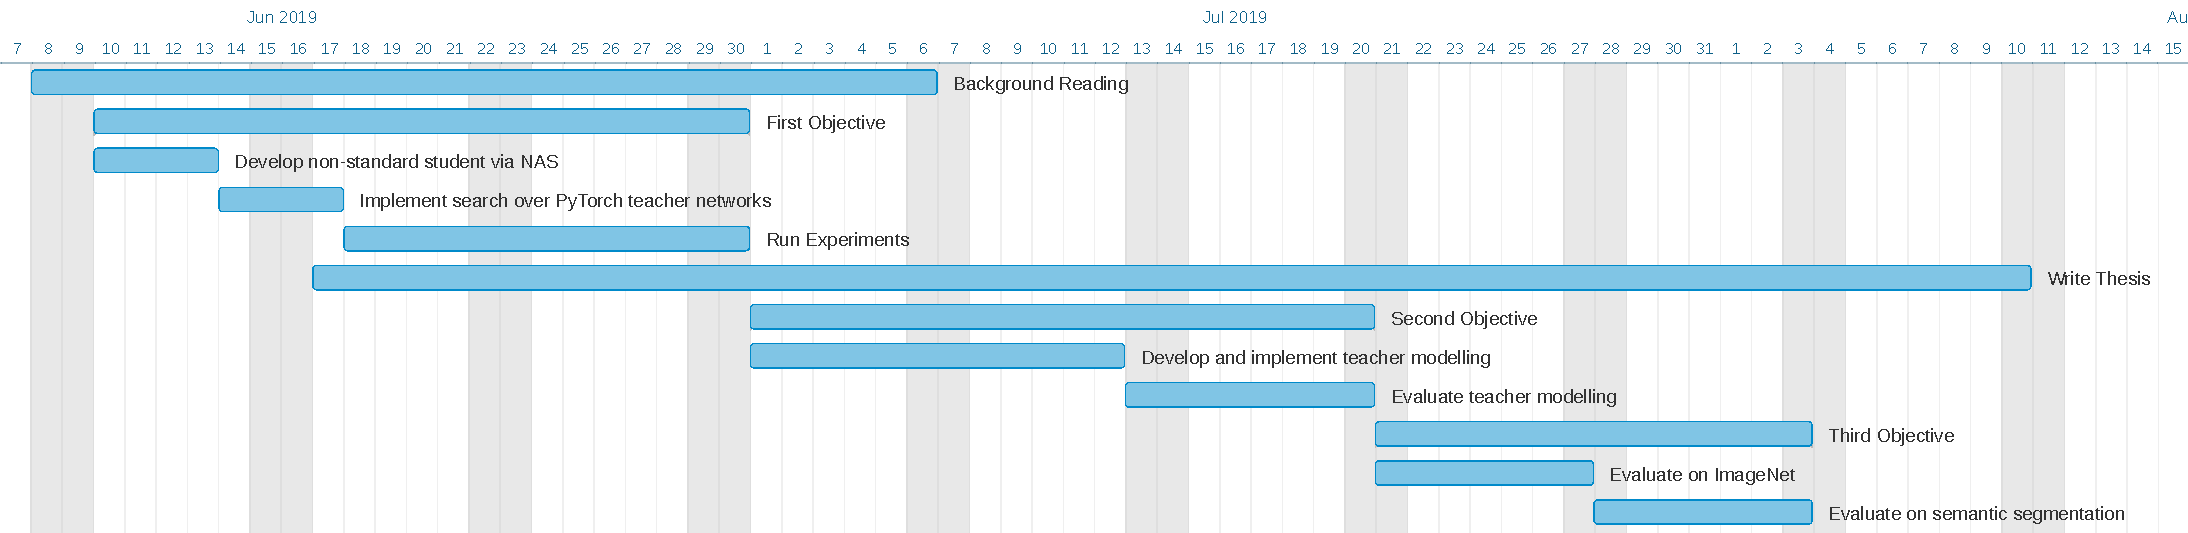
\includegraphics[scale=0.45]{Gantt.pdf}
\end{figure}

\begin{table}[htbp]
    \begin{center}
        \begin{tabular}{|c|c|l|}
        \hline
        \textbf{Milestone} & \textbf{Week} & \textbf{Description} \\
        \hline
        $M_1$ & 2 & Implement experimental setup for standard teacher architectures\\
        $M_2$ & 2 & Experiments with standard teachers completed\\
        $M_3$ & 5 & Teacher modelling implementation completed \\
        $M_4$ & 7 & Teacher modelling evaluation \\
        $M_4$ & 10 & Evaluation on alternative task and data\\
        \hline
        \end{tabular} 
    \end{center}
    \caption{Milestones defined in this project.}
    \label{fig:milestones}
\end{table}

\begin{table}[htbp]
    \begin{center}
        \begin{tabular}{|c|c|l|}
        \hline
        \textbf{Deliverable} & \textbf{Week} & \textbf{Description} \\
        \hline
        $D_1$ & 6 & Experimental results for standard teacher networks\\
        $D_2$ & 8 & Teacher modelling algorithm and results\\
        $D_3$ & 10 & Thesis \\
        \hline
        \end{tabular} 
    \end{center}
    \caption{List of deliverables defined in this project.}
    \label{fig:deliverables}
\end{table}


%                Now build the reference list
\bibliographystyle{unsrt}   % The reference style
%                This is plain and unsorted, so in the order
%                they appear in the document.

{\small
\bibliography{main}       % bib file(s).
}
\end{document}

